\section{Classical learning}
In this Chapter we are going to explain the Methods k-nearest-neighbours and support vector machine. Also we are going to briefly introduce decision trees because we are using them in Chapter 5 for AdaBoost.

%%%%%%%%%%%%%%%%%%%%%%%%%%%%%%%%%%%%%%%%%%%%%%%%%%%%%%%%%

\subsection{KNN}
The KNN algorithm assumes that similar things exist in close proximity. In other words, similar things are near to each other.

The straight-line distance (Euclidean distance) is a popular and familiar choice to measure the distance between two samples.
Note that there are other ways of calculating distance, and one way might be preferable depending on the problem we are solving. Other possibilities to measure the distance could be e.g. Manhattan or Hamming.
In the following picture the black dot could be classified as - if we only compare with the next neighbour. But if one chooses to compare with the three nearest neighbours it the dot would be classified as +, because two dots would be + and only one would be -. It is important to select a "good" amount of neighbours to classify. An example for this can be found in the next picture where the black dot is near to an (probably) outlier. If k would be chosen as 1 then the black dot would be classified as + but it would probably be -.

\begin{figure}[hbtp]
	\centering
	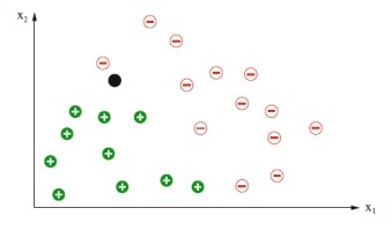
\includegraphics[scale=0.8]{knn1}
	\caption{K-Nearest Neighbors}
	% \vspace{-20pt}
	\label{fig:Datensatz - unbearbeitet}
\end{figure}

\begin{figure}[hbtp]
	\centering
	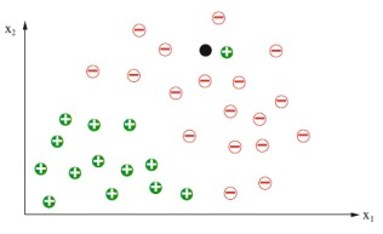
\includegraphics[scale=0.8]{knn2}
	\caption{K-Nearest Neighbors}
	% \vspace{-20pt}
	\label{fig:Datensatz - unbearbeitet}
\end{figure}
 
 
\textbf{Sources:}
\begin{itemize}
\item scikit-learn: \hyperlink{https://scikit-learn.org/stable/modules/generated/sklearn.neighbors.KNeighborsClassifier.html}{https://scikit-learn.org/stable/modules/generated/sklearn.neighbors.KNeighborsClassifier.html} \\
\hyperlink{https://scikit-learn.org/stable/modules/neighbors.html}{https://scikit-learn.org/stable/modules/neighbors.html}
\item Wikipedia: Nächste-Nachbarn-Klassifikation \hyperlink{https://de.wikipedia.org/wiki/Nächste-Nachbarn-Klassifikation}{https://de.wikipedia.org/wiki/Nächste-Nachbarn-Klassifikation}
\end{itemize} 
%%%%%%%%%%%%%%%%%%%%%%%%%%%%%%%%%%%%%%%%%%%%%%%%%%%%%%%%%

\subsection{Decision Trees}

(Classification-) Decision tree

The data will be divided by yes/no questions. This is done by selecting the question such that the best information gain is created(spliting the data via a feature which can seperate the different lables best). There are different methods to measure the entrophy from which the information gain can be calculated. A common approach is to calculate the Gini-index. For more information please have a look at the scources. In the following picture one can see a decision tree with depth 8. Trees tend to overfit if one let them grow to their maximum depth, so there are methods to prevent this from happening(e.g. pruning).

\begin{figure}[hbtp]
	\centering
	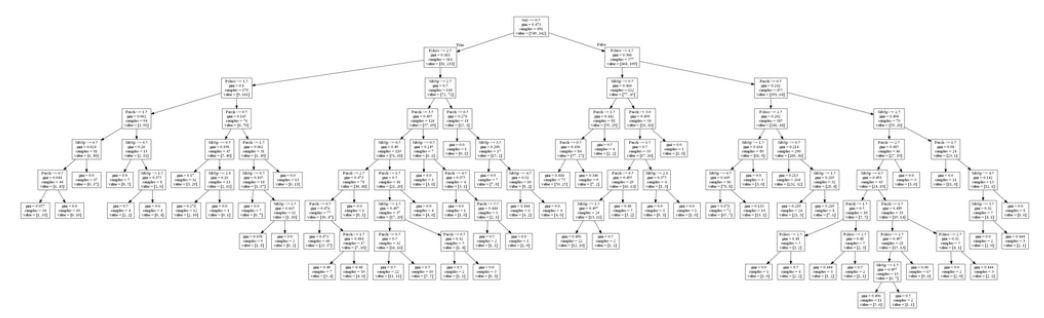
\includegraphics[scale=0.5]{tree}
	\caption{Decision Tree}
	% \vspace{-20pt}
	\label{fig:Datensatz - unbearbeitet}
\end{figure}


Decision Trees can used for ensemble methods (Random forest, adaboost,...). We refere to Chapter 5.

\textbf{Sources:}
\begin{itemize}
\item scikit-learn: \hyperlink{https://scikit-learn.org/stable/modules/tree.html}{https://scikit-learn.org/stable/modules/tree.html} \\
\hyperlink{https://scikit-learn.org/stable/modules/generated/sklearn.tree.DecisionTreeClassifier.html}{https://scikit-learn.org/stable/modules/generated/sklearn.tree.DecisionTreeClassifier.html}
\item Wikipedia: Entscheidungsbaum \hyperlink{https://de.wikipedia.org/wiki/Entscheidungsbaum}{https://de.wikipedia.org/wiki/Entscheidungsbaum}
\end{itemize}

%%%%%%%%%%%%%%%%%%%%%%%%%%%%%%%%%%%%%%%%%%%%%%%%%%%%%%%%%%%
%%%%%%%%%%%%%%%%%%%%%%%%%%%%%%%%%%%%%%%%%%%%%%%%%%%%%%%%%%%
\subsection{Support Vector Machine}
\subsubsection{Introduction}

Support Vector Machines (SVM) are supervised learning algorithms for classification.
They are one of the most widely used supervised learning algorithms. 
SVMs offer a high accuracy when it comes to classification.
The idea behind a SVM is to find a hyperplane that seperates classes of datapoints with a large margin. Where the margin is the smallest distance between the closest datapoint $x$ of one class and the hyperplane (therefore the name 'support vector'). Because of this feature the SVM is sometimes also called \textbf{large margin classifier}.
The so called kernel trick can be applied when non linear data has to be classified.

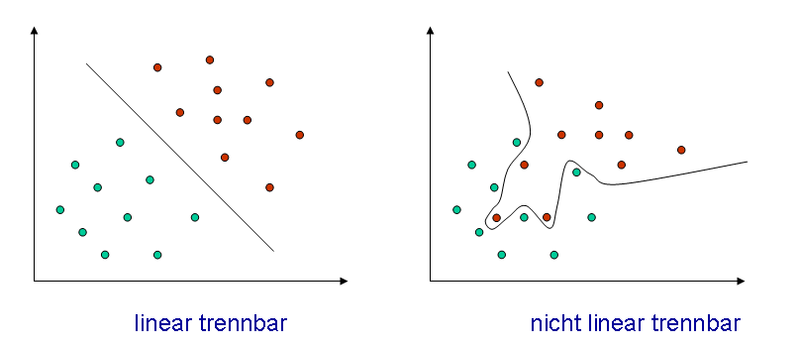
\includegraphics[scale=0.5]{Images/svm.png}


\subsubsection{Linear Support Vector Machines}

This is one of the algorithms implemented in this project and there is a future section devoted to it. 

For a short introduction, assume the Support Vector Machine algorithm is being used for a binary classification problem~$\mathcal{Y} = \{-1, 1\}$, that the training set has~$\mathcal{X} \subset \mathbb{R}^d$ and the subsets~$X_{-1} = \{ x^i\in \mathcal{X} \colon y^i = -1 \}$, ~$X_{1} = \{ x^i\in \mathcal{X} \colon y^i = 1 \}$ can be the separated by an affine hyperplane. Under these assumptions, the hypothesis space is the set of affine hyperplanes in~$\mathbb{R}^d$ that separate the training data and not all possible affine hyperplanes, as in Linear regression.

While in Linear Regression the empirical risk adds an error for each element in the data set, in SVMs the error of a given hyperplane is the sum~$\delta_{-} + \delta_{+}$, where~$\delta_{-}$ is the minimum distance between the hyperplane and an input point which would be classified as~$-1$ and~$\delta_{+}$ is defined analogously, for an input point which would be classified as~$1$.


\subsubsection{Mathematics behind SVMs}
For given input data $X = \{x_{1}, ..., x_{m}\}$, with $x_{i} \in \mathbb{R}^n$ and matching result vector $Y = \{y_{1}, ..., y_{m}\}$, with $y_{i} \in \{-1, 1\}$. We want a classifier \\ $h: \mathbb{R}^{n} \rightarrow \{-1, 1\}$ such that $h(x) = $ $\begin{cases*} 1 & ,if $ w^{T} x + b  > 0$,\\ -1& ,if $w^{T} x+b < 0$.\end{cases*}$ with $w \in \mathbb{R}^{n}$ and $b \in \mathbb{R}$. We want h to be correct for most samples. This formulation leads to the following primal problem: \\
$min_{w,b,s} \frac{1}{2} w w^T + C \sum_{i = 1}^m s_{i}$, \\
s.t.: $y_i (w^T x_i + b ) \geq 1 - s_i$, $s_i \geq 0$. \\
Where $s_i$ are the so called slack variables that should denote the distance from the correct margin if a point is misclassified. \\
Intuitively we want to maximize the margin what results in minimizing $||w||^2$ including a penalty when something is misclassified.
$C$ controlls the strength of the misclassification penaly. One could view it as a inverse regularization parameter. A large C results in overfitting and a smaller C results in a "smoother" fit.\\
The dual problem to the above Primal problem is: \\
$min_{\lambda} \frac{1}{2} \lambda^T Q \lambda - e^T \lambda$ \\
s.t.: $y^T \lambda = 0$ and $0 \leq \lambda_{i} \leq C$ for all $i = 1,...,m$.
The entries of the matrix $Q \in \mathbb{R}^{m \times m}$ are given by $Q_{i, j} = y_i y_j \langle x_i, x_j \rangle$. \\
This shows that the minimization only depends on the scalar product of $x_i$ and $x_j$ and we can apply the kernel trick. Instead of the standard scalar product we can use a kernel function $K(x_i, x_j)$.

\subsubsection{In our case}
We use the python library sklearn, which can easily be installed via pip.
First we get the training data and split it into training and test data.\\
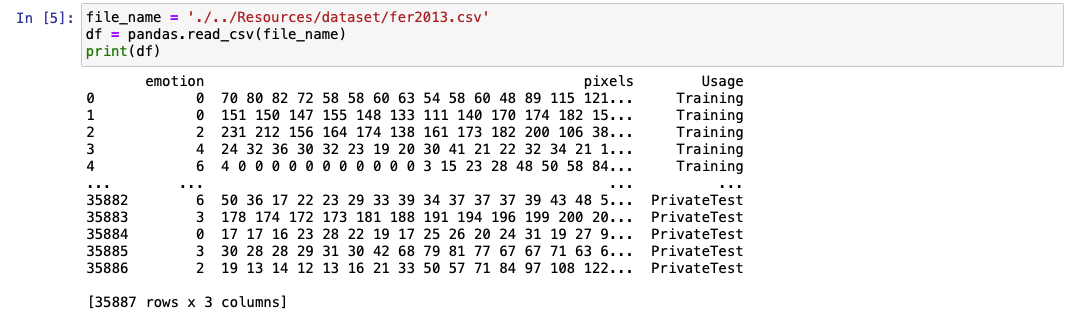
\includegraphics[scale=0.4]{Images/trainingdata.png} \\
Next we fit the model to the training data for the chosen parameters and safe it with the pickle model. \\
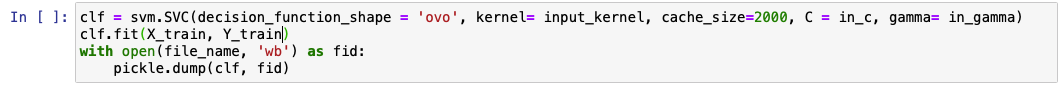
\includegraphics[scale=0.4]{Images/trainmodel.png} \\
Now the model can give a prediction on new images. \\
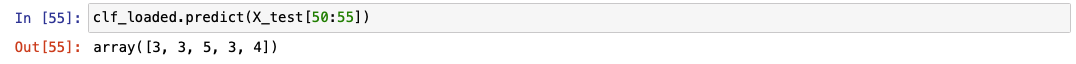
\includegraphics[scale=0.4]{Images/svm_prediction.png}

\textbf{Sources:}
\begin{itemize}
\item Martin Lotz: \textit{Mathematics of Machine Learning}. Lecture Notes, Warwick (UK), 2020.
\item scikit-learn: \hyperlink{https://scikit-learn.org/stable/modules/generated/sklearn.svm.SVC.html}{https://scikit-learn.org/stable/modules/generated/sklearn.svm.SVC.html} \\
\hyperlink{https://scikit-learn.org/stable/modules/svm.html}{https://scikit-learn.org/stable/modules/svm.html}
\item Coursera: Machine Learning, by Stanford University \\ \hyperlink{https://www.coursera.org/learn/machine-learning/home/welcome}{https://www.coursera.org/learn/machine-learning/home/welcome}
\item Wikipedia: Support vector machine.\hyperlink{https://en.wikipedia.org/wiki/Support\_vector\_machine}{https://en.wikipedia.org/wiki/Support\_vector\_machine}
\end{itemize}


%%%%%%%%%%%%%%%%%%%%%%%%%%%%%%%%%%%%%%%%%%%%%%%%%%%%%%


\newpage